\chapter{Dari Bunga Menjadi Buah}\label{ch:g5:flower-to-fruit}

\Cref{ch:g3:flowers-fruits-seeds} mengamati \omterm{def:g3:flowers-fruits-seeds:parts}{bunga} ceri menjadi \omterm{prop:g3:flowers-fruits-seeds:transform}{buah}
ceri dan meninggalkan satu pertanyaan terbuka: \emph{apa yang
sesungguhnya terjadi} ketika sebutir \omterm{def:g3:flowers-fruits-seeds:parts}{serbuk sari} mendarat di \omterm{def:g3:flowers-fruits-seeds:parts}{putik}?
Tahun ini, berbekal gagasan \omterm{def:g5:flower-to-fruit:steps}{pembuahan} dari
\cref{ch:g4:animal-reproduction} dan \omterm{def:g5:first-look-at-cells:cell}{sel} dari
\cref{ch:g5:first-look-at-cells}, kita dapat membuka permesinan \omterm{def:g3:flowers-fruits-seeds:parts}{bunga}
itu dengan benar.

\section{Bunga punya bagian jantan dan bagian betina}

\begin{proposition}[Dua peran bunga dalam satu]\label{prop:g5:flower-to-fruit:roles}
Perkembangbiakan pada \omterm{def:g1:plants-around-us:plant}{tumbuhan} berbunga adalah reproduksi
\emph{seksual}, persis dalam pengertian
\cref{def:g4:animal-reproduction:sexual} --- dan kebanyakan \omterm{def:g3:flowers-fruits-seeds:parts}{bunga}
membawa kedua perannya sekaligus:
\begin{itemize}
  \item \emph{\omterm{def:g3:flowers-fruits-seeds:parts}{benang sari}} adalah bagian \omterm{def:g4:animal-reproduction:sexual}{jantan}: tiap butir
        \emph{\omterm{def:g3:flowers-fruits-seeds:parts}{serbuk sari}} membawa \omterm{def:g5:first-look-at-cells:cell}{sel} kelamin \omterm{def:g4:animal-reproduction:sexual}{jantan} \omterm{def:g1:plants-around-us:plant}{tumbuhannya};
  \item \emph{\omterm{def:g3:flowers-fruits-seeds:parts}{putik}} adalah bagian \omterm{def:g4:animal-reproduction:sexual}{betina}: jauh di dalamnya terbaring
        \emph{bakal biji}\index{bakal biji}, masing-masing memuat
        sebuah \omterm{def:g4:animal-reproduction:sexual}{sel telur}.
\end{itemize}
``Calon \omterm{def:g2:from-seed-to-plant:seed}{biji}'' pada \cref{def:g3:flowers-fruits-seeds:parts} sekarang
punya nama yang sesungguhnya: \omterm{prop:g5:flower-to-fruit:roles}{bakal biji}, yang menunggu untuk
dibuahi.
\end{proposition}
\admitted

\begin{remark}[Rancangan yang sama dengan hewan]\label{rem:g5:flower-to-fruit:sameplan}
\omterm{def:g5:first-look-at-cells:cell}{Sel} \omterm{def:g4:animal-reproduction:sexual}{jantan}, \omterm{def:g4:animal-reproduction:sexual}{sel telur}, \omterm{def:g5:flower-to-fruit:steps}{pembuahan}: perbendaharaan kata
\cref{ch:g4:animal-reproduction} diterjemahkan kata demi kata.
\omterm{prop:g5:first-look-at-cells:principle}{Kesatuan kehidupan} sekali lagi
(\cref{prop:g5:first-look-at-cells:principle}) --- \omterm{def:g3:flowers-fruits-seeds:parts}{bunga} aster dan
lumba-lumba berkembang biak atas satu rancangan dasar yang sama,
seberbeda apa pun tampak permesinannya.
\end{remark}

\section{Penyerbukan, lalu pembuahan}

\begin{definition}[Kedua langkahnya]\label{def:g5:flower-to-fruit:steps}
Membuat sebutir \omterm{def:g2:from-seed-to-plant:seed}{biji} membutuhkan dua langkah yang berbeda:
\begin{enumerate}
  \item \emph{penyerbukan}\index{penyerbukan}: sebutir \omterm{def:g3:flowers-fruits-seeds:parts}{serbuk sari}
        mengembara dari sebuah \omterm{def:g3:flowers-fruits-seeds:parts}{benang sari} ke puncak sebuah \omterm{def:g3:flowers-fruits-seeds:parts}{putik} ---
        dibawa \omterm{prop:g3:sorting-living-things:groups}{serangga}
        (\cref{prop:g3:flowers-fruits-seeds:transform}) atau oleh
        angin;
  \item \emph{pembuahan}\index{pembuahan pada tumbuhan}: butir yang
        mendarat itu menumbuhkan sebuah buluh halus \emph{turun
        menembus \omterm{def:g3:flowers-fruits-seeds:parts}{putiknya}}; melaluinya, \omterm{def:g5:first-look-at-cells:cell}{sel} \omterm{def:g4:animal-reproduction:sexual}{jantannya} mencapai sebuah
        \omterm{prop:g5:flower-to-fruit:roles}{bakal biji} lalu bergabung dengan \omterm{def:g4:animal-reproduction:sexual}{sel telurnya}.
\end{enumerate}
Penyerbukan adalah perjalanannya; pembuahan adalah pertemuannya.
\end{definition}

\begin{omfigure}
\begin{tikzpicture}
  \node[anchor=south west, inner sep=0] (img) at (0,0)
    {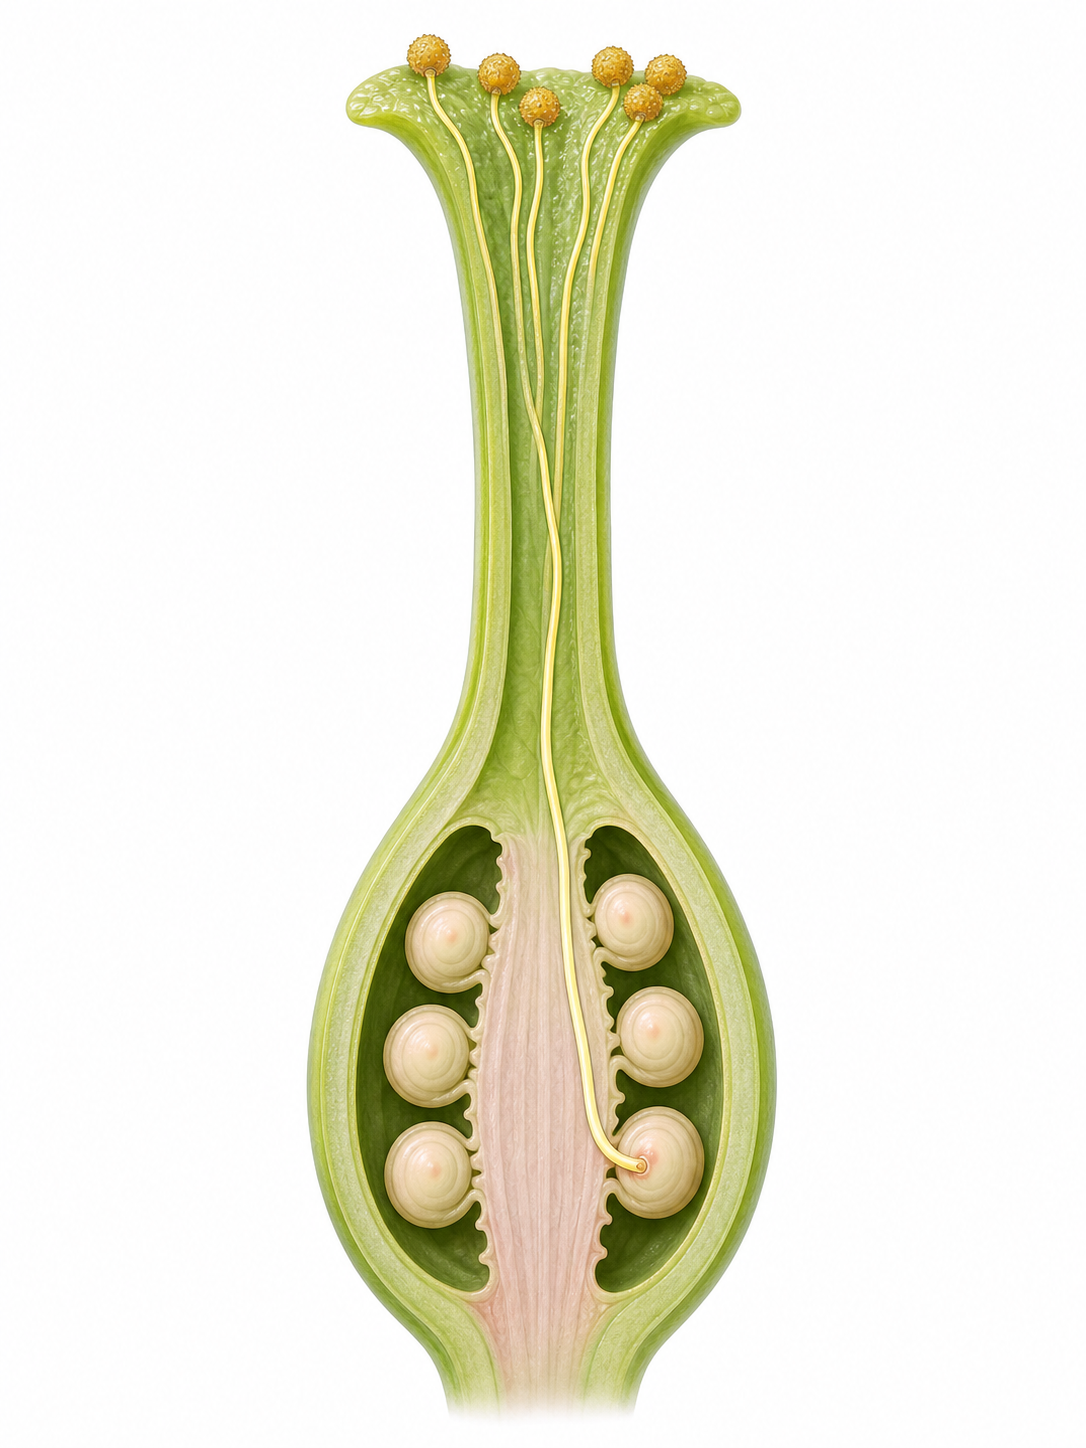
\includegraphics[width=0.42\linewidth]{images/book1/ai/fig-pistil-tube.png}};
  \begin{scope}[x={(img.south east)}, y={(img.north west)},
      every node/.style={font=\small}]
    \draw[omProp, thick] (0.62,0.95) -- (0.80,0.97)
      node[right, align=left, omProp]
      {butir serbuk sari mendarat:\\ penyerbukan};
    \draw[omProp, thick] (0.53,0.55) -- (0.78,0.60)
      node[right, align=left, omProp]
      {buluh serbuk sarinya\\ tumbuh turun};
    \draw[omDef, thick] (0.36,0.26) -- (-0.05,0.30)
      node[left, align=right, omDef]
      {bakal biji, masing-masing\\ dengan sel telur};
    \draw[omDef, thick] (0.62,0.15) -- (0.80,0.11)
      node[right, align=left, omDef]
      {sel jantannya tiba:\\ pembuahan};
  \end{scope}
\end{tikzpicture}

{\small Di dalam \omterm{def:g3:flowers-fruits-seeds:parts}{putik}: sebutir \omterm{def:g3:flowers-fruits-seeds:parts}{serbuk sari} yang mendarat menumbuhkan
buluhnya turun ke sebuah \omterm{prop:g5:flower-to-fruit:roles}{bakal biji}, dan \omterm{def:g5:flower-to-fruit:steps}{pembuahan} terjadi di dasarnya.}
\end{omfigure}

\begin{example}[Mengapa bunga yang tak dikunjungi gugur]\label{ex:g5:flower-to-fruit:unvisited}
Aturan kebun \omterm{prop:g3:flowers-fruits-seeds:transform}{buah} pada \cref{rem:g3:flowers-fruits-seeds:bees}
sekarang punya mekanismenya: tanpa kunjungan, tidak ada \omterm{def:g3:flowers-fruits-seeds:parts}{serbuk sari} di
\omterm{def:g3:flowers-fruits-seeds:parts}{putiknya}; tanpa \omterm{def:g3:flowers-fruits-seeds:parts}{serbuk sari}, tidak ada buluh, tidak ada \omterm{def:g5:flower-to-fruit:steps}{pembuahan}; dan
\omterm{def:g3:flowers-fruits-seeds:parts}{bunga} yang tidak terbuahi layu seluruhnya --- tidak ada \omterm{def:g3:flowers-fruits-seeds:parts}{putik} yang
membengkak, tidak ada \omterm{prop:g3:flowers-fruits-seeds:transform}{buah} ceri. Langkah yang hilang itu tidak
terlihat, hanya perjalanan sebuah \omterm{def:g5:first-look-at-cells:cell}{sel} menuruni sebuah buluh --- tetapi
dahan yang kosong pada bulan Juli cukup terlihat.
\end{example}

\section{Sesudah pertemuannya: biji dan buah}

\begin{proposition}[Tiap bagian menjadi apa]\label{prop:g5:flower-to-fruit:becomes}
Sesudah \omterm{def:g5:flower-to-fruit:steps}{pembuahan}, perubahan pada
\cref{prop:g3:flowers-fruits-seeds:transform} berjalan dengan
ketepatan yang baru:
\begin{itemize}
  \item tiap \emph{\omterm{prop:g5:flower-to-fruit:roles}{bakal biji} yang terbuahi} menjadi sebutir
        \emph{\omterm{def:g2:from-seed-to-plant:seed}{biji}} --- \omterm{def:g1:plants-around-us:plant}{tumbuhan} mungil di dalamnya
        (\cref{def:g2:from-seed-to-plant:seed}) tumbuh dari \omterm{def:g4:animal-reproduction:sexual}{sel telur}
        yang terbuahi, persis seperti seekor \omterm{def:g1:animals-around-us:animal}{hewan} tumbuh dari \omterm{def:g4:animal-reproduction:sexual}{sel
        telurnya} sendiri
        (\cref{ex:g5:first-look-at-cells:one});
  \item \emph{\omterm{def:g3:flowers-fruits-seeds:parts}{putik}} di sekelilingnya membengkak menjadi
        \emph{\omterm{prop:g3:flowers-fruits-seeds:transform}{buah}};
  \item \omterm{def:g3:flowers-fruits-seeds:parts}{mahkota bunga} dan \omterm{def:g3:flowers-fruits-seeds:parts}{benang sarinya}, yang tugasnya selesai, layu
        lalu gugur.
\end{itemize}
\end{proposition}
\admitted

\begin{example}[Menghitung biji]\label{ex:g5:flower-to-fruit:pips}
Belah sebuah apel melintang: lima bilik kecil, beberapa \omterm{def:g2:from-seed-to-plant:seed}{biji} di
masing-masing. Tiap \omterm{def:g2:from-seed-to-plant:seed}{biji} adalah satu \omterm{prop:g5:flower-to-fruit:roles}{bakal biji} yang dicapai satu
buluh \omterm{def:g3:flowers-fruits-seeds:parts}{serbuk sari}. Sebuah apel yang miring sebelah dengan bilik kosong
di satu sisinya menceritakan \omterm{def:g3:flowers-fruits-seeds:parts}{bunga} yang buruk \omterm{def:g5:flower-to-fruit:steps}{penyerbukannya} --- terlalu
sedikit butir yang mendarat untuk membuahi semua \omterm{prop:g5:flower-to-fruit:roles}{bakal bijinya}, dan
\omterm{prop:g3:flowers-fruits-seeds:transform}{buahnya} membengkak tidak merata.
\end{example}

\begin{omfigure}
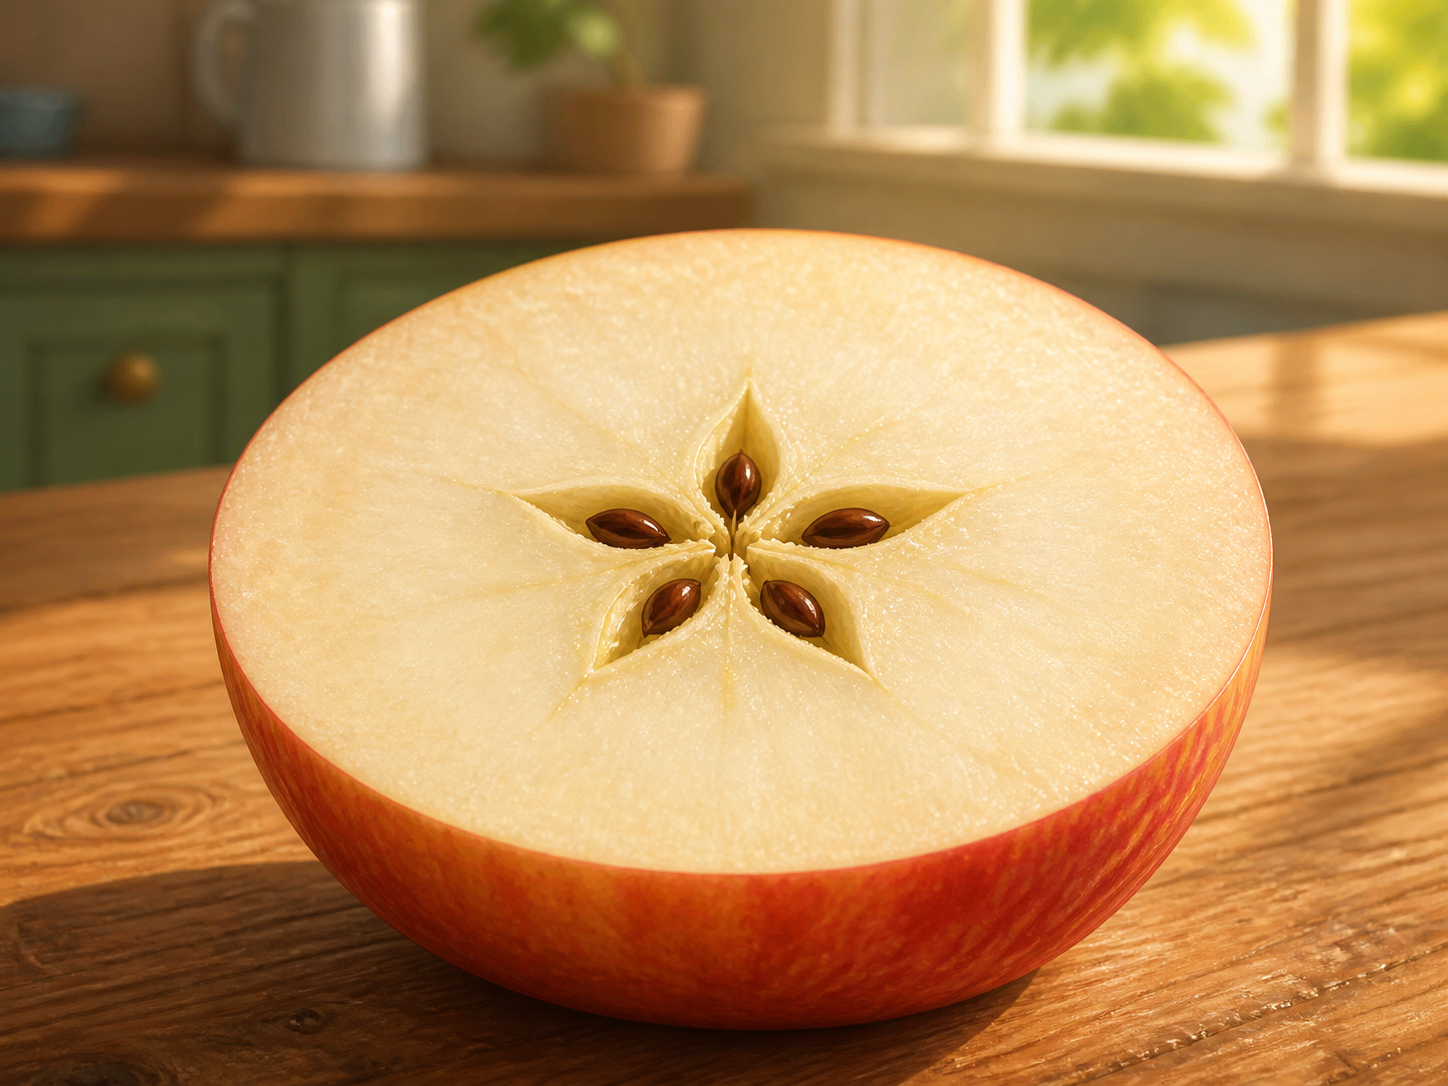
\includegraphics[width=0.56\linewidth]{images/book1/ai/g5-flower-applepips.png}

{\small Apel yang dibelah melintang: lima bilik dalam bentuk bintang,
dan di dalamnya \omterm{def:g2:from-seed-to-plant:seed}{bijinya} --- satu \omterm{def:g2:from-seed-to-plant:seed}{biji} bagi tiap \omterm{prop:g5:flower-to-fruit:roles}{bakal biji} yang
dicapai sebuah buluh \omterm{def:g3:flowers-fruits-seeds:parts}{serbuk sari}.}
\end{omfigure}

\begin{example}[Serbuk sari yang dibawa angin]\label{ex:g5:flower-to-fruit:wind}
Rerumputan, gandum dan pohon hazel tidak punya \omterm{def:g3:flowers-fruits-seeds:parts}{mahkota bunga}, tidak
punya bau harum, tidak punya nektar --- tidak ada yang ditawarkan
kepada pengunjung. \omterm{def:g3:flowers-fruits-seeds:parts}{Serbuk sarinya} menumpang \emph{angin}: dibuat dalam
jumlah amat besar, sehalus debu, dilemparkan ke udara untuk mendarat
di tempat yang ditentukan nasib. Siasat itu menukar ketepatan dengan
jumlah --- logika awan \omterm{def:g4:plants-without-seeds:spore}{spora} pada
\cref{rem:g4:plants-without-seeds:sporeseed}, yang dimainkan dengan
\omterm{def:g3:flowers-fruits-seeds:parts}{serbuk sari}. (\omterm{def:g3:flowers-fruits-seeds:parts}{Serbuk sari} di udara itulah, sambil lalu, yang
menggelitik hidung yang alergi pada bulan Juni.)
\end{example}

\begin{method}[Mendiagnosis tumbuhan yang tidak berbuah]\label{met:g5:flower-to-fruit:diagnose}
Sebuah \omterm{def:g1:plants-around-us:plant}{tumbuhan} berbunga lebat tetapi tidak menghasilkan \omterm{prop:g3:flowers-fruits-seeds:transform}{buah}.
Tanyakan berurutan:
\begin{enumerate}
  \item Apakah penyerbuknya mencapainya? (Di dalam ruangan, terjaring,
        tidak ada \omterm{prop:g3:sorting-living-things:groups}{serangga} di sekitarnya, minggu-minggu berbunga yang
        dingin dan berhujan?)
  \item Kalau tidak, serbukilah dengan tangan: sentuhkan kuas lembut
        pada \omterm{def:g3:flowers-fruits-seeds:parts}{benang sari} sekuntum \omterm{def:g3:flowers-fruits-seeds:parts}{bunga}, lalu pada \omterm{def:g3:flowers-fruits-seeds:parts}{putik} \omterm{def:g3:flowers-fruits-seeds:parts}{bunga} yang
        lain;
  \item apakah embun beku atau kerusakan mematikan \omterm{def:g3:flowers-fruits-seeds:parts}{bunganya} sebelum
        \omterm{prop:g5:flower-to-fruit:roles}{bakal bijinya} sempat dibuahi
        (\cref{exo:g3:flowers-fruits-seeds:9})?
  \item Kalau \omterm{prop:g3:flowers-fruits-seeds:transform}{buahnya} sekarang terbentuk, permesinan \omterm{def:g1:plants-around-us:plant}{tumbuhannya}
        sehat --- hanya perjalanan pada langkah 1 yang gagal.
\end{enumerate}
\end{method}

\section{Latihan}

\begin{exercise}[$\star$]\label{exo:g5:flower-to-fruit:1}
Bagian \omterm{def:g3:flowers-fruits-seeds:parts}{bunga} yang mana yang \omterm{def:g4:animal-reproduction:sexual}{jantan}, dan apa yang dibuatnya? Yang mana
yang \omterm{def:g4:animal-reproduction:sexual}{betina}, dan apa yang terbaring di dalamnya?
\end{exercise}

\begin{exercise}[$\star$]\label{exo:g5:flower-to-fruit:2}
Definisikan \omterm{def:g5:flower-to-fruit:steps}{penyerbukan} dan \omterm{def:g5:flower-to-fruit:steps}{pembuahan}, lalu sebutkan mana yang datang
lebih dahulu.
\end{exercise}

\begin{exercise}[$\star$]\label{exo:g5:flower-to-fruit:3}
Ceritakan perjalanan satu butir \omterm{def:g3:flowers-fruits-seeds:parts}{serbuk sari}, dari \omterm{def:g3:flowers-fruits-seeds:parts}{benang sari} sampai
\omterm{def:g4:animal-reproduction:sexual}{sel telur}, dalam empat langkah.
\end{exercise}

\begin{exercise}[$\star$]\label{exo:g5:flower-to-fruit:4}
Sesudah \omterm{def:g5:flower-to-fruit:steps}{pembuahan}: tiap \omterm{prop:g5:flower-to-fruit:roles}{bakal biji} yang terbuahi menjadi apa? \omterm{def:g3:flowers-fruits-seeds:parts}{Putiknya}
menjadi apa? Apa yang terjadi pada \omterm{def:g3:flowers-fruits-seeds:parts}{mahkota bunganya}?
\end{exercise}

\begin{exercise}[$\star$]\label{exo:g5:flower-to-fruit:5}
Tiap \omterm{def:g2:from-seed-to-plant:seed}{biji} apel itu apa, dalam perbendaharaan kata bab ini? Apa yang
diceritakan sebuah apel yang miring sebelah dengan bilik yang kosong?
\end{exercise}

\begin{exercise}[$\star$]\label{exo:g5:flower-to-fruit:6}
Bagaimana rerumputan dan pohon hazel diserbuki tanpa \omterm{def:g3:flowers-fruits-seeds:parts}{mahkota bunga},
bau harum atau nektar? Apa harga metode mereka?
\end{exercise}

\begin{exercise}[$\star$]\label{exo:g5:flower-to-fruit:7}
Mengapa \omterm{def:g3:flowers-fruits-seeds:parts}{bunga} yang tidak dikunjungi \omterm{prop:g3:sorting-living-things:groups}{serangga} biasanya tidak
menghasilkan \omterm{prop:g3:flowers-fruits-seeds:transform}{buah}? Sebutkan langkah yang hilang.
\end{exercise}

\begin{exercise}[$\star$]\label{exo:g5:flower-to-fruit:8}
Cobalah (dengan tanaman berbunga di balkon atau ambang jendela):
serbukilah dua \omterm{def:g3:flowers-fruits-seeds:parts}{bunga} dengan tangan memakai kuas lembut, seperti pada
\cref{met:g5:flower-to-fruit:diagnose}, lalu tandailah keduanya dengan
benang. Apakah \omterm{def:g3:flowers-fruits-seeds:parts}{bunga} yang ditandai lebih sering menghasilkan \omterm{prop:g3:flowers-fruits-seeds:transform}{buah}
daripada yang lain?
\end{exercise}

\begin{exercise}[$\star\star$]\label{exo:g5:flower-to-fruit:9}
Daftarkan kesejajaran antara perkembangbiakan \omterm{def:g1:plants-around-us:plant}{tumbuhan} dan \omterm{def:g1:animals-around-us:animal}{hewan}: \omterm{def:g5:first-look-at-cells:cell}{sel}
\omterm{def:g4:animal-reproduction:sexual}{jantan}, \omterm{def:g4:animal-reproduction:sexual}{sel telur}, \omterm{def:g5:flower-to-fruit:steps}{pembuahan}, \omterm{def:g5:first-look-at-cells:cell}{sel} pertama individu barunya. Pada \omterm{def:g3:flowers-fruits-seeds:parts}{bunga},
masing-masing bertempat di mana?
\end{exercise}

\begin{exercise}[$\star\star$]\label{exo:g5:flower-to-fruit:10}
Musim semi seorang petani ceri terasa dingin dan berhujan: lebah nyaris
tidak terbang selama dua minggu, walaupun tidak ada embun beku dan
pohonnya berbunga dengan megah. Ramalkan panen bulan Julinya lalu
jelaskan dengan \cref{def:g5:flower-to-fruit:steps}.
\end{exercise}

\begin{exercise}[$\star\star\star$]\label{exo:g5:flower-to-fruit:11}
Seorang penanam tomat di rumah kaca memasang sebuah sarang lebah
bombus di dalamnya, walaupun tidak ada \omterm{def:g3:flowers-fruits-seeds:parts}{bunga} di luar yang dapat
dicapai dari rumah kaca yang tertutup rapat itu. Dengan memakai bab
ini, jelaskan persis jasa apa yang dijual lebah bombusnya --- dan
mengapa kipas yang mengembuskan udara melewati tanamannya dapat
sebagian menggantikannya bagi tomat (yang \omterm{def:g3:flowers-fruits-seeds:parts}{serbuk sarinya} mudah
terguncang lepas), sedangkan bagi pohon ceri tidak dapat.
\end{exercise}
